\section{Ausgangslage}
\label{sec:Ausgangslage}

\subsection{Szenario}

\begin{wrapfigure}{l}{0.55\textwidth}
  \begin{center}
    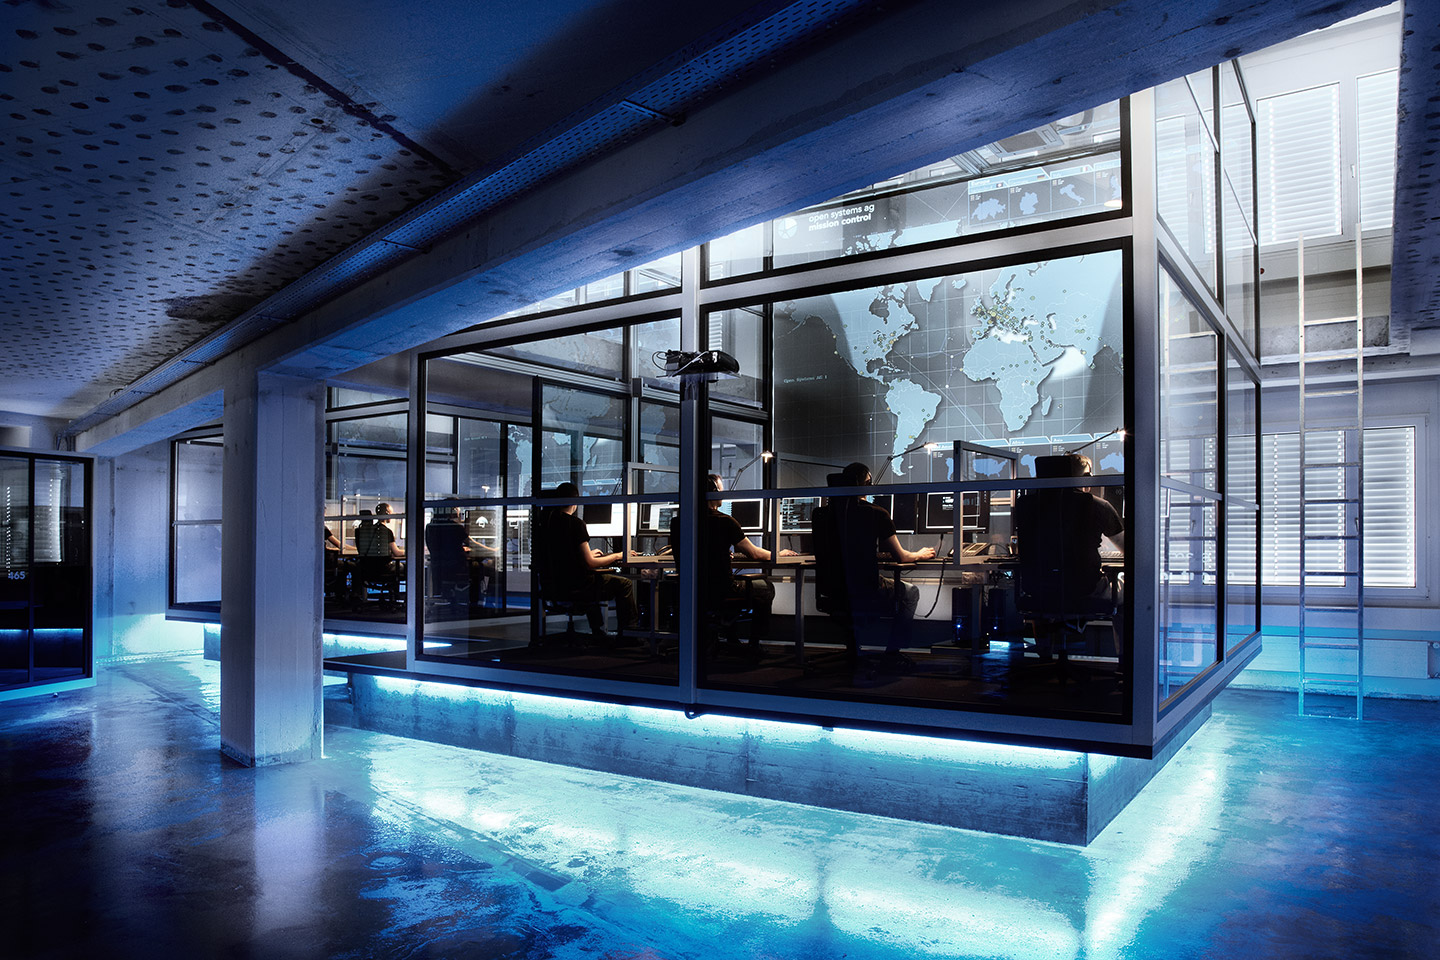
\includegraphics[clip,scale=0.15]{mainpart/anforderungen/img/gallery_mc_01}
    \caption{Mission Control Center}
  \end{center}
\end{wrapfigure}

Die Firma \osag betreibt ein weltweites Netz von \acs{IPSec} \acs{VPN} Verbindungen. Die Kunden der \osag kommen unter anderem aus den Branchen: Finanzen, Versicherungen, Regierung sowie Detail Handel. Daher ist es für \osag sehr wichtig dass die Verbindungen konstant überwacht werden. Zu diesem Zweck wird auch ein Mission Control Center betrieben dass den Betrieb der \acs{VPN} Tunnels 24/7 überwacht. Dieses Mission Control Center\footnotemark[1] ist zuständig dass periodische Tests der Verbindungsqualität gemacht werden sowie akkute Probleme direkt erkannt und behoben werden. Das manuelle Überprüfen von Paket-Verlusten und bestimmen von Fragmentierungsproblem nimmt viel Zeit in Anspruch. Mit dem \tool soll dies automatisiert werden so dass mit weniger Arbeit eine noch besser Verbindungsqualität angeboten werden kann.

\footnotetext[1]{Bild: \url{http://open.ch}}